\chapter{Introduction}
% \label{sec:chapter1}

%
The rapid growth of the world population and the limited ability to supply non-renewable energy is leading to a rise of power demand, especially in developing countries. The current energy demand requires an intensive usage of fossil energy causing environmental pollution, as well as climate change. \\

Indeed, the increase of global temperature and the worsening of the air quality are posing a real problem for the environment. The changes observed in Earth’s climate are primarily driven by human activities, particularly fossil fuel burning. The biggest disadvantage of fossil fuels is that during the process of combustion in addition to produce energy, greenhouse gases (\gls{GHG}) are emitted \cite{greenhousegasemissions}. \\
Normally the solar energy from the sun would hit the earth and then part of this energy bounce back to the space, but these gases trap the heat from the sun in the atmosphere, increasing the earth temperatures. \\

In order to improve the situation, the 2015 Paris Agreement set an ambition to limit global warming to well below $\SI{2}{\degreeCelsius}$ above pre-industrial levels and pursue efforts to limit it to $\SI{1.5}{\degreeCelsius}$ - in part by pursuing net carbon neutrality by 2050. The substantial reduction of global greenhouse gas emissions (including \gls{CarbonDiox})  will limit the increase of global temperature \cite{french_conference}. \\
Countries were asked to go through a process of decarbonization: the reduction of carbon dioxide emissions through the use of low carbon power sources. \\
%Renewable energy production has low or no waste products such as \gls{CarbonDiox} or other chemical pollutants.  \\
% These low carbon power sources usually are renewable energies such as sun, wind, geothermal heat and other natural sources.
These sources convert the energy coming through naturals elements (sun, wind, geothermal heat) in another form of energy, electricity for example, with low or no waste products such as \gls{CarbonDiox} or other chemical pollutants. \\

\begin{figure}[H]
\centering
    % 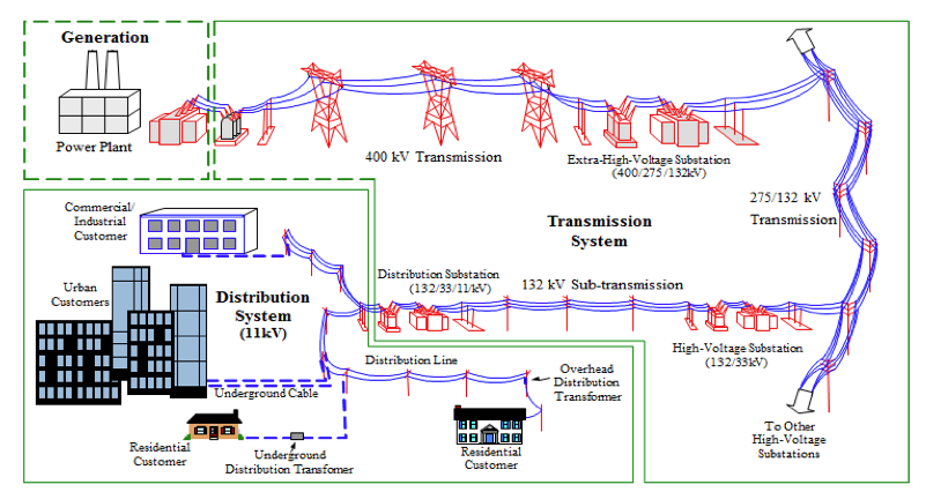
\includegraphics[width=.9\linewidth]{images/DN/HighMediumLowV.png}
    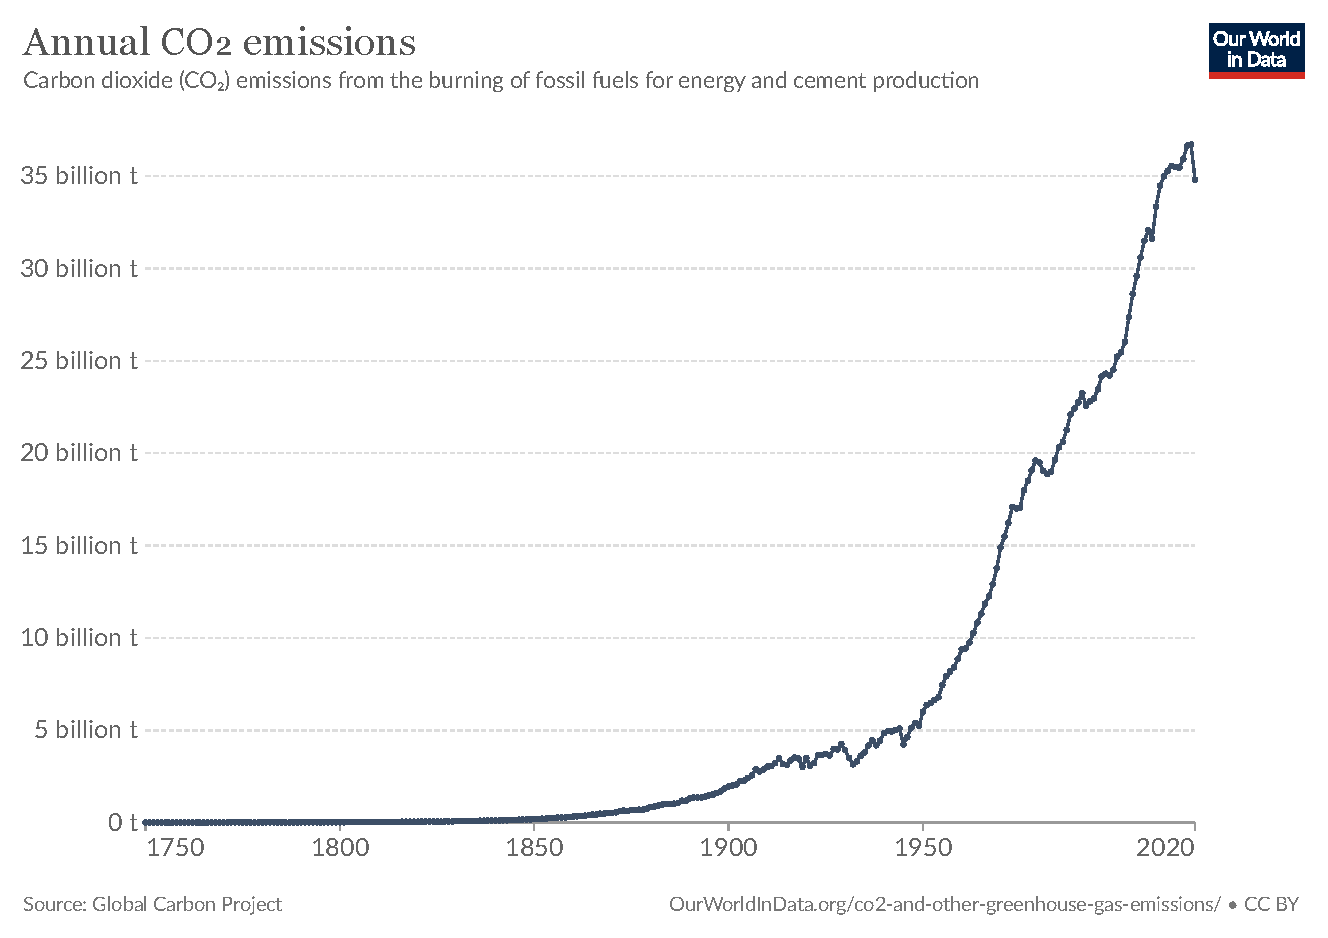
\includegraphics[width=.6\linewidth]{images/Introduction/annual-co2-emissions-per-country.pdf}
\caption[\gls{CarbonDiox} production]{World \gls{CarbonDiox} production over the years \cite{C02prod}}
% \label{fig:gym_anm_net}
\end{figure}

Thanks to this emerging trend of decarbonization, more and more renewable power energy devices are introduced in the distribution networks \cite{owidenergy}. High penetration of these renewables devices bring in some technical complications for the distribution of power and voltage in the grids. \\
The networks, that have been designed around the conventional centralized energy production, have to adapt to the new generators in the system. It is possible to say that the distribution networks are moving from unidirectional power flow (from the distribution system to the consumers) to a bidirectional power flow (in this case the consumers are also producers and the exceed energy can be transported from the consumers to the distribution system. They are also known as prosumers \cite{prosumers}). This switch from unidirectional to bidirectional power flow requires a smarter system that can handle in an efficient way the generation and distribution of voltage.\\

In the literature, this smarter way to control a distribution system is known as active network management (\gls{ANM}) and it refers to the design of control schemes that modulate the generators, the loads, and the distributed energy storages (\glspl{DES}), as well as other elements like switches, connected to the grid. \\


\section{Aim of the thesis}
\label{sec:aimthesis}
The aim of this thesis is to exploit data-driven approaches to forecast the future distribution of voltages based on historical measurements in a medium-voltage distribution system using machine learning techniques, in particular deep learning models. Predicting over voltages problems of lines would allow avoiding possible consequences related to these issues. 

% \section{Research methods}

\section{Thesis outline}
% Chapter 2 provides
% \\
% Chapter 3 ...

